
\documentclass[openany,11pt]{homework}

\coursename{ELEN 4903 Machine Learning (Spring 2018)} % DON'T CHANGE THIS

\studname{Pratyus Pati}    % YOUR NAME GOES HERE
\studmail{pp2636@columbia.edu}% YOUR UNI GOES HERE
\hwNo{2}                   % THE HOMEWORK NUMBER GOES HERE

% Uncomment the next line if you want to use \includegraphics.
\usepackage{graphicx}

\begin{document}
\maketitle

\section*{Problem 1(a)}

\begin{align}
\hat{\pi}_{ML} & = \operatornamewithlimits{arg\,max}_{\pi} p(y_1, y_2, ..., y_n \mid \pi) \\
			   & = \operatornamewithlimits{arg\,max}_{\pi} \pi^{n\mu_y}(1-\pi)^{n-n\mu_y} \\
			   & = \operatornamewithlimits{arg\,max}_{\pi} \ln(\pi^{n\mu_y}(1-\pi)^{n-n\mu_y}) \\
			   & = \operatornamewithlimits{arg\,max}_{\pi} [(n\mu_y) (\ln \pi)] + [(n - n\mu_y)(\ln (1-\pi))]
\end{align}

On taking the derivative w.r.t. $\pi$\\
\begin{align}
\frac{\partial }{\partial \pi} [(n\mu_y) (\ln \pi)] + [(n - n\mu_y)(\ln (1-\pi))]
& = \left[n\mu_y \frac{\partial \ln \pi}{\partial \pi}\right] + \left[(n - n\mu_y)\left(\frac{\partial \ln(1-\pi)}{\partial \pi}\right)\right] \\
& = \frac{n\mu_y}{\pi} -\frac{n-n\mu_y}{1-\pi}
\end{align}

On setting the partial derivative w.r.t $\pi$ as 0 to get $\hat{\pi}_{ML}$,
\begin{align}
\frac{n\mu_y}{\hat{\pi}_{ML}} -\frac{n-n\mu_y}{1-\hat{\pi}_{ML}} & = 0 \\
\Rightarrow n\mu_y(1-\hat{\pi}_{ML}) - (n-n\mu_y)(\hat{\pi}_{ML}) & = 0 \\
\Rightarrow n\mu_y - n\mu_y\hat{\pi}_{ML} - n\hat{\pi}_{ML} + n\mu_y\hat{\pi}_{ML} & = 0 \\
\Rightarrow n\mu_y - n\hat{\pi}_{ML} & = 0 \\
\Rightarrow \hat{\pi}_{ML} & = \mu_y = \frac{\sum_{i=1}^{n} y_i}{n}
\end{align}

\section*{Problem 1(b)}

\begin{align}
\hat{\theta_y^{1}}_{ML} & = \operatornamewithlimits{arg\,max}_{\theta_y^{1}} p(x_{1,1}, x_{2,1}, ..., x_{n, 1} \mid \theta_y^{1})
\end{align}

Splitting the data into separate classes: \\
\begin{align}
I_y & = \{i \mid y_i = y\} \\
n_y & = \mid I_y \mid
\end{align}

Using this to represent the probability distribution $p(x_{1,1}, x_{2,1}, ..., x_{n, 1} \mid \theta_y^{1})$:

\begin{align}
\hat{\theta_y^{1}}_{ML} & = \operatornamewithlimits{arg\,max}_{\theta_y^{1}} p(x_{1,1}, x_{2,1}, ..., x_{n, 1} \mid \theta_y^{1}) \\
                        & = \operatornamewithlimits{arg\,max}_{\theta_y^{1}} \prod_{i=1}^{n} p(x_{i,1} \mid \theta_{y_i}^{1}) \\
                        & = \operatornamewithlimits{arg\,max}_{\theta_y^{1}} \sum_{i=1}^{n} \ln p(x_{i,1} \mid \theta_{y_i}^{1}) \\
                        & = \operatornamewithlimits{arg\,max}_{\theta_y^{1}} \sum_{i=1}^{n} \ln (\theta_{y_i}^{1}^{x_{i,1}})(1-\theta_{y_i}^{1})^{1-x_{i,1}} \\
                        & = \operatornamewithlimits{arg\,max}_{\theta_y^{1}} \sum_{i=1}^{n} x_{i,1} \ln (\theta_{y_i}^{1}) + (1-x_{i,1}) \ln (1-\theta_{y_i}^{1})
\end{align}

On differentiating with respect to $\theta_{y}^{1}$, and setting it to 0 to get ${\theta_{y}^{1}}_{ML}$:

\begin{align}
\sum_{i \in I_y} \frac{x_{i,1}}{{\theta_{y}^{1}}_{ML}} - \frac{1 - x_{i,1}}{1 - {\theta_{y}^{1}}_{ML}} & = 0 \\
\Rightarrow \frac{\sum_{i \in I_y} x_{i,1}}{{\theta_{y}^{1}}_{ML}} - \frac{n_y - \sum_{i \in I_y} x_{i,1}}{1 - {\theta_{y}^{1}}_{ML}} & = 0 \\
\Rightarrow {\theta_{y}^{1}}_{ML} & = \frac{\sum_{i \in I_y} x_{i,1}}{n_y}
\end{align}

Therefore:
\begin{align}
{\theta_{0}^{1}}_{ML} & = \frac{\sum_{i \in I_0} x_{i,1}}{n_0}\\
{\theta_{1}^{1}}_{ML} & = \frac{\sum_{i \in I_1} x_{i,1}}{n_1}
\end{align}

\section*{Problem 1(c)}

\begin{align}
\hat{\theta_y^{2}}_{ML} & = \operatornamewithlimits{arg\,max}_{\theta_y^{1}} p(x_{1,2}, x_{2,2}, ..., x_{n, 2} \mid \theta_y^{2})
\end{align}

Splitting the data into separate classes: \\
\begin{align}
I_y & = \{i \mid y_i = y\} \\
n_y & = \mid I_y \mid
\end{align}

Using this to represent the probability distribution $p(x_{1,2}, x_{2,2}, ..., x_{n, 2} \mid \theta_y^{2})$:

\begin{align}
\hat{\theta_y^{2}}_{ML} & = \operatornamewithlimits{arg\,max}_{\theta_y^{2}} p(x_{1,2}, x_{2,2}, ..., x_{n, 2} \mid \theta_y^{2}) \\
                        & = \operatornamewithlimits{arg\,max}_{\theta_y^{2}} \prod_{i=1}^{n} p(x_{i,1} \mid \theta_{y_i}^{2}) \\
                        & = \operatornamewithlimits{arg\,max}_{\theta_y^{1}} \sum_{i=1}^{n} \ln p(x_{i,2} \mid \theta_{y_i}^{2}) \\
                        & = \operatornamewithlimits{arg\,max}_{\theta_y^{1}} \sum_{i=1}^{n} \ln (\theta_{y_i}^{2}){x_{i,2}}^{-(\theta_{y_i}^{2} + 1)} \\
                        & = \operatornamewithlimits{arg\,max}_{\theta_y^{1}} \sum_{i=1}^{n} \ln (\theta_{y_i}^{2}) - (\theta_{y_i}^{2} + 1) \ln (x_{i,2})
\end{align}

On differentiating with respect to $\theta_{y}^{1}$, and setting it to 0 to get ${\theta_{y}^{2}}_{ML}$:

\begin{align}
\sum_{i \in I_y} \frac{1}{{\theta_{y}^{2}}_{ML}} - {\ln (x_{i,2})} & = 0 \\
\Rightarrow {\theta_{y}^{2}}_{ML} & = \frac{n_y}{\sum_{i \in I_y} \ln x_{i,2}}
\end{align}

Therefore:
\begin{align}
{\theta_{0}^{2}}_{ML} & = \frac{n_0}{\sum_{i \in I_0} \ln x_{i,2}}\\
{\theta_{1}^{2}}_{ML} & = \frac{n_1}{\sum_{i \in I_1} \ln x_{i,2}}
\end{align}

\section*{Problem 2(a)}
\begin{figure}[h]
	\centering
	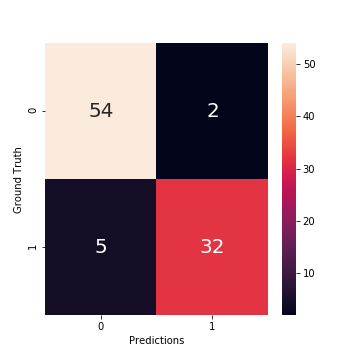
\includegraphics[width= 0.5\textwidth]{2a}
	\caption{Confusion Matrix}
\end{figure}

TestAccuracy: $(54+32)/93 = 86/93 = 92.47\%$

\section*{Problem 2(b)}
\begin{figure}[!h]
	\centering
	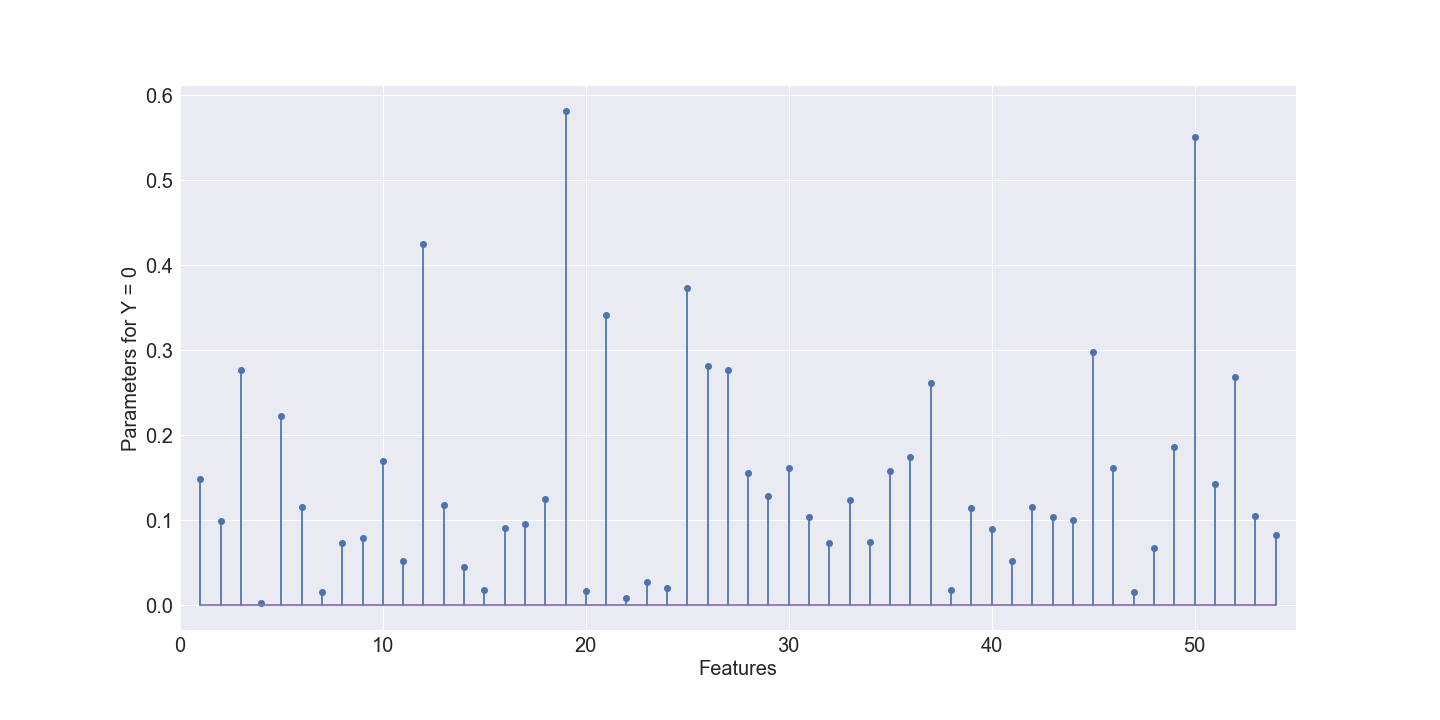
\includegraphics[width= 0.9\textwidth]{2b1}
	\caption{Stem Plot for Y = 0}
\end{figure}

\begin{figure}[!h]
	\centering
	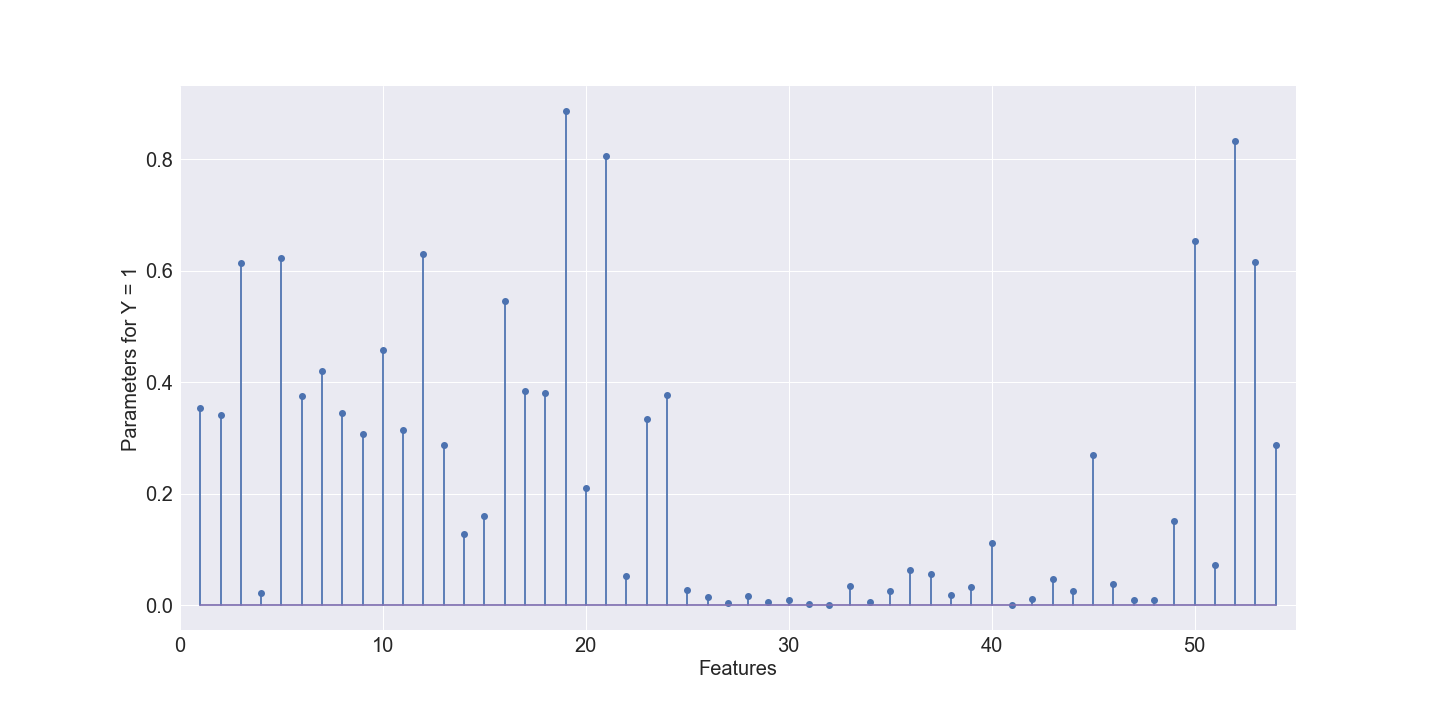
\includegraphics[width=0.9\textwidth]{2b2}
	\caption{Stem Plot for Y = 1}
\end{figure}

According to the spambase.names, the features are either a word frequency or a character frequency. Since the features follow a Bernoulli distribution, the probability $\theta_y^{i}$ represents the contribution of the presence of $i^{th}$ feature to  the probability that the a particular data sample belongs to a class y. Mathematically, $\theta_y^{i} = \frac{\sum_{j \in I_y} x_{j,i}}{n_y}$.

From the stem plot, feature 16 (word\_freq\_free - the frequency of the word `free' in the document) has a $\theta_0^{16}$ of 0.091 which is the likelihood of occurence of the word `free' in the not-spam class. Additionally, feature 52 (char\_freq\_! - the frequency of the character `!' in the document) has a $\theta_0^{52}$ of 0.269 which is the relative likelihood of occurence of the character `!' in the not-spam class.

From the stem plot, feature 16 (word\_freq\_free - the frequency of the word `free' in the document) has a $\theta_1^{16}$ of 0.545 which means that there is a moderate likelihood of the occurence of the word `free' in the spam class. Additionally, feature 52 (char\_freq\_! - the frequency of the character `!' in the document) has a $\theta_1^{52}$ of 0.833 which means that there is a high likelihood of the occurence of the character `!' in the spam class.

For predicting the class based on just observing a single feature, we can calculate the odds as $\frac{p(x \mid y = 1)p(y = 1)}{p(x \mid y = 0)p(y = 0)}$. From the calculations, $p(y = 1) \approx 0.4$. Therefore, if $x_{i,16} = 1$, the odds turn out to be $\frac{0.545 x 0.4}{0.091 x 0.6} = \frac{4}{1}$. Therefore, all other things kept constant, if a mail has the word 'free', it is 4 times more likely to be classified as spam than not-spam. Similarily, for $x_{i,52} = 1$ the odds turn out to be $\frac{0.833 x 0.4}{0.269 x 0.6} = \frac{2}{1}$. Therefore, all other things kept constant, if a mail has the character `!', it is 2 times more likely to be classified as spam than not-spam.

\section*{Problem 2(c)}
\begin{figure}[h]
	\centering
	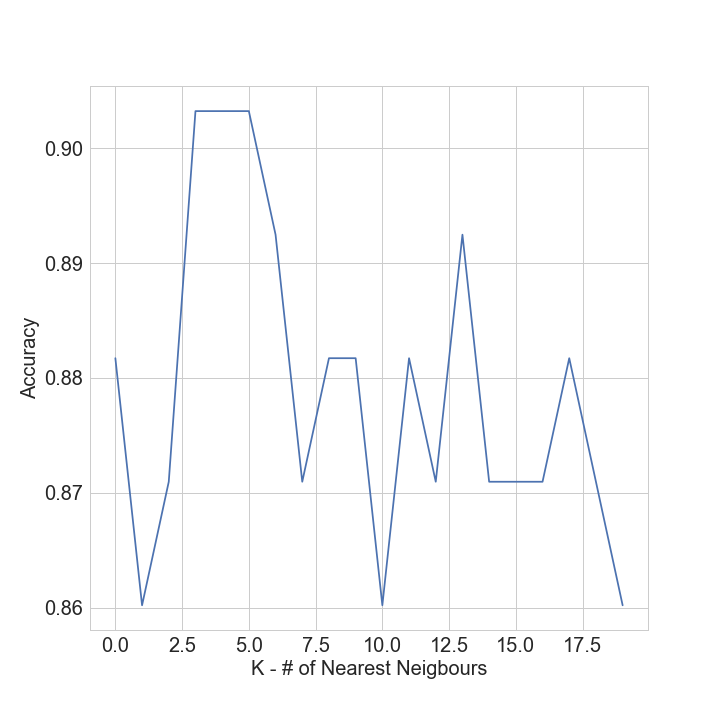
\includegraphics[width=\textwidth]{2c}
	\caption{Variation of Classification Accuracy vs. K - No. of Nearest Neigbours}
\end{figure}

Observation: There isn't any clear trend of accuracy vs. K. However, the maximum test accuracy can be seen to occur at k = 3, 4 or 5

\section*{Problem 2(d)}
\begin{figure}[h]
	\centering
	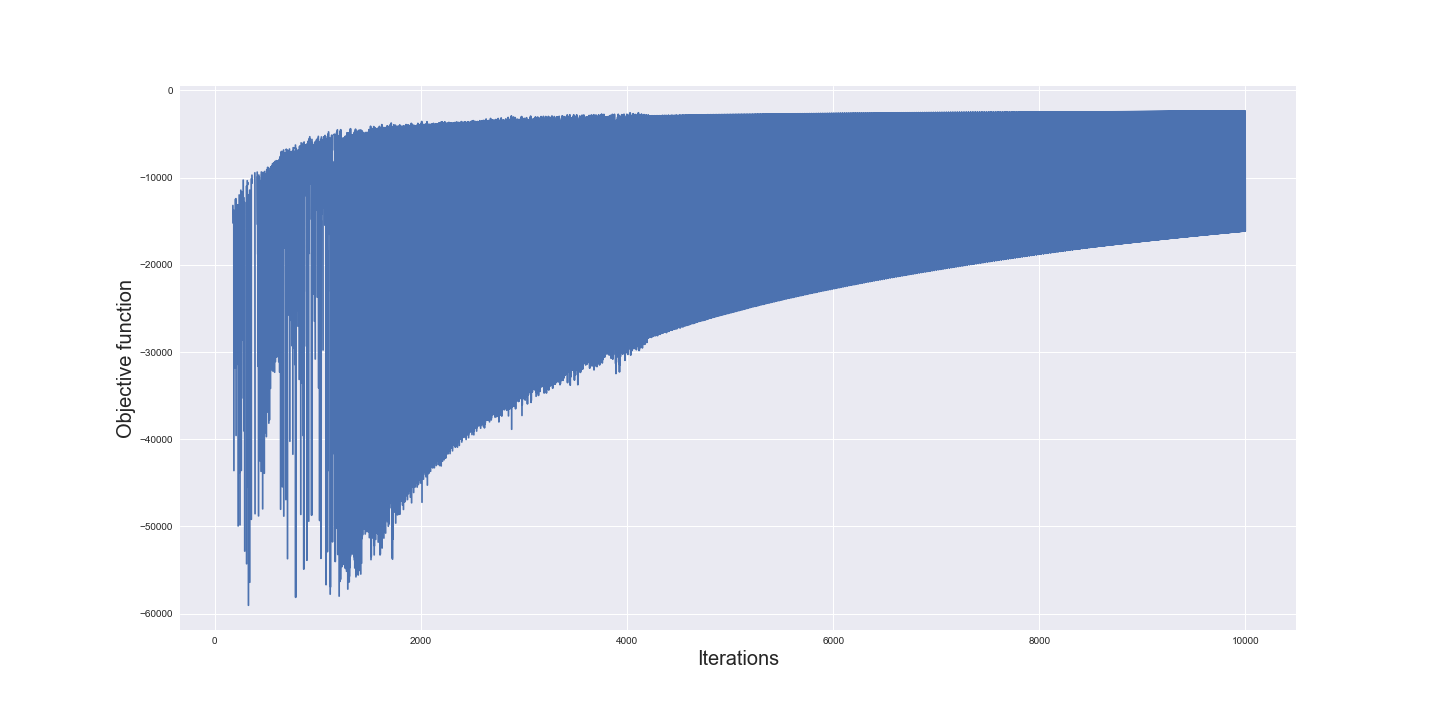
\includegraphics[width=\textwidth]{2d}
	\caption{Optimization of Objective Function over multiple iterations}
\end{figure}

Note: This result was obtained using scipy.special.expit() for calculating exponentials for higher values.
\\
\\
Observation: There is no clear pattern. This could be as a result of projecting the results of a multi-dimensional optimization onto a 2D plane. However, it can be seen that the objective function is generally increasing with the number of iterations.
\\
\\
Test Accuracy after training for 10,000 iterations: 82.79\%

\section*{Problem 2(e)}
\begin{figure}[h]
	\centering
	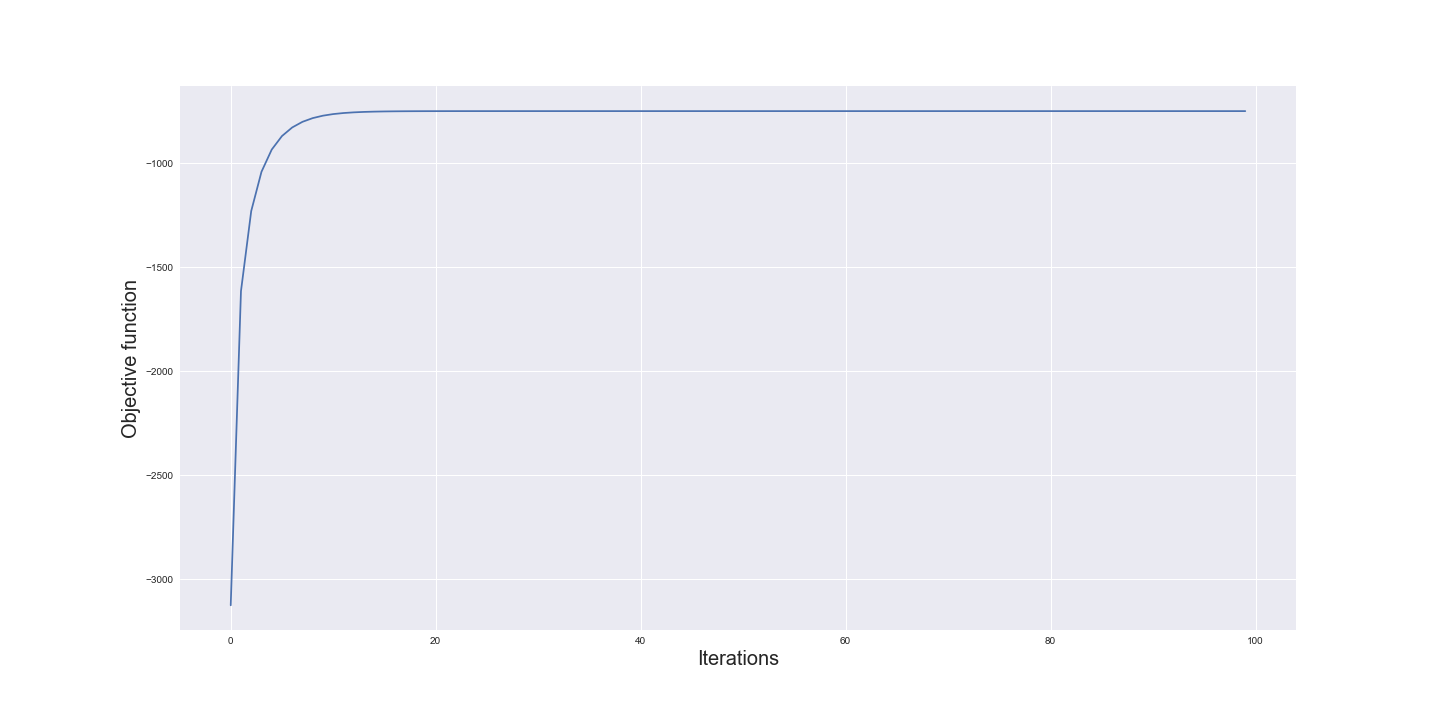
\includegraphics[width=\textwidth]{2e}
	\caption{Optimization of Objective Function over multiple iterations using Newton's Method}
\end{figure}

Observation: Using Newton's method for gradient ascent results in faster optimization - achieving a better test accuracy in 100 iterations as compared to the accuracy achieved using the vanilla gradient ascent after 10,000 iterations.
\\
\\
Test accuracy after training for 100 iterations: 91.39\%
\end{document}
